% !TEX root = ../main.tex

% Indicate the main file. Must go at the beginning of the file.

%---------------------------------------------------------------------
% CHAPTER TEMPLATE
%---------------------------------------------------------------------


\chapter{Methode} % Main chapter title
\label{ChapterX} % Change X to a consecutive number; for referencing this chapter elsewhere, use \ref{ChapterX}

%---------------------------------------------------------------------
% SECTION Busauslastung messen
%---------------------------------------------------------------------

\section{Busauslastung messen}
\textcolor{red}{Ein kurze Zusammenfasung, wie anhand einer Messug auf dem Bus mit Matlab ein Buslauslastung gemessen und ausgewertet wurde. Outcome präsentieren}

Um zu beurteilen, ob Bluetooth Low Energy (BLE) eine geeignete Lösung für die Übertragung von Telegrammen vom Sniffer zum Endgerät darstellt, wurde ein Versuch unternommen, die Busauslastung mittels Oszilloskop zu analysieren. Ziel war es, abzuschätzen, ob die dabei gewonnenen effektiven Nutzdaten über BLE übertragen werden können. Gleichzeitig sollte geprüft werden, ob eine direkte Übertragung aller Rohdaten möglich ist oder ob eine Filterung der Telegramme erforderlich wäre.

Für die Analyse wurden zwei Messungen durchgeführt: eine unter Normallast und eine unter Volllast. Die Volllast wurde simuliert, indem der Depot-Diagnosespeicher auf dem Fahrzeugdisplay angezeigt wurde. Dies führte dazu, dass der Speicher die entsprechenden Daten über den Bus an das Display sendete, was kurzfristig zu einer höheren Auslastung führte.

Die Messungen wurden mit einem Picoscope 2207B durchgeführt, während die anschließende Auswertung mit MATLAB realisiert wurde.

\subsection{Messaufbau}

Der Messaufbau ist in Abbildung \ref{fig:MessaufbauBusauslastungMessen} dargestellt. Um die Busauslastung zu messen, wurde die MVB-Leitung, die normalerweise von Gerät zu Gerät durchgeschleift ist, an einer geeigneten Stelle unterbrochen und ein Leitungsaufteiler eingefügt. Dies ermöglichte den direkten Zugriff auf die differentiellen Leitungen des Busses mit dem Picoscope. Der MVB-Loop wurde dabei wieder geschlossen, sodass keine Geräte vom Bus abgetrennt wurden. Die gemessenen Daten wurden über eine USB-Schnittstelle an einen Laptop übertragen und dort mit der Pico-Software aufgezeichnet.

\begin{figure}[H]
    \centering
    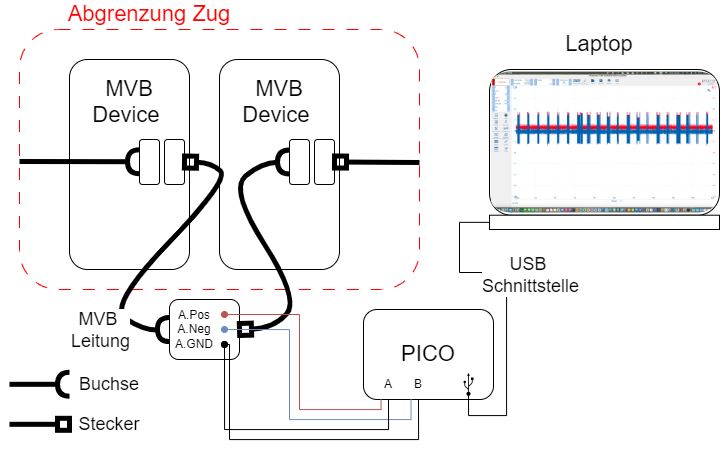
\includegraphics[width=0.8\linewidth]{Figures/Chap3/Busauslastung/Messaufbau_PICO_IC2000.png}
    \caption{Messaufbau Busauslastung messen}
    \label{fig:MessaufbauBusauslastungMessen}
\end{figure}

Die erfassten Daten wurden anschließend in das MATLAB-Dateiformat (.mat) exportiert. Die Struktur der MATLAB-Datei ist in Abbildung \ref{fig:MatlabFileStruktur} dargestellt. Die Variablen \textit{A} und \textit{B} entsprechen den Messpunkten des Picoscope, während \textit{Tinterval} die Zeit zwischen zwei Messpunkten angibt. 

\begin{figure}[H]
    \centering
    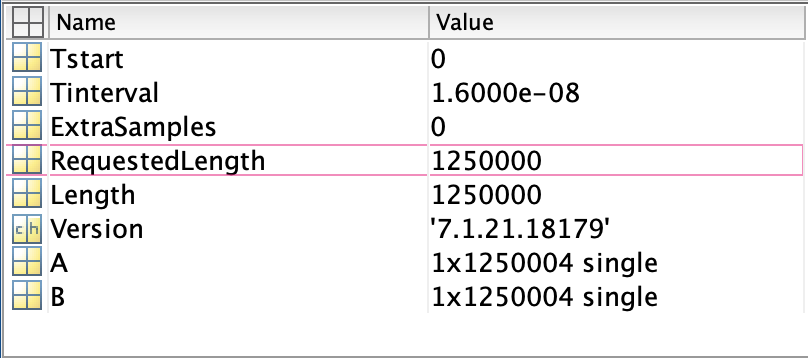
\includegraphics[width=0.5\linewidth]{Figures/Chap3/Busauslastung/Matlab_file_struktur.png}
    \caption{Matlab File Struktur}
    \label{fig:MatlabFileStruktur}
\end{figure}

Der Messaufbau blieb für die Messungen unter Normallast und Volllast identisch. Um die Volllast zu simulieren, wurde der Befehl zur Anzeige der Depot-Diagnosedaten auf dem Fahrzeugdisplay ausgelöst, bevor die Messung gestartet wurde. Der Zeitraum zwischen der Eingabe des Befehls und der Darstellung der Daten auf dem Display beträgt etwa 5 Sekunden.

\subsection{Matlab Auswertung}

\subsubsection{Variablen initialisieren}

\subsubsection{Delimiter erkennen}

\subsubsection{Nulldurchgänge}

\subsubsection{Auswertung Effektive Nutzdaten}







%----------------------------------------------------------------------
% SECTION Wahl der Hardware
%----------------------------------------------------------------------

\section{Design eigener Sniffer}
\textcolor{red}{Wie wurde der Sniffer aufgebaut. Schematischer Verlauf von D-Sub9 bis Endgerät soll aufgezeigt und erklärt werden.}

Für den ersten Entwurf des Sniffers wurde eine Anforderungsliste erstellt, in welcher die Fest- wie auch Wunschanforderungen definiert sind. In einem ersten Entwurf wurde schematisch dargestellt in welcher Reifenfolge welche Aufgabe won welcher Hardware durchgeführt werden soll. 

Dieser schematische Entwurf (siehe Abbildung x) zeigt die verschiedene Hardware auf und wie diese verbunden sind. Dabei wurden direkt die technischen Anforderungen, welche durch den MVB vorgegeben sind, im Schema dargestellt.

Um auf dem Differentiellen Signal ein einziges zu machen welches

Anhand dem ersten Entwurf, wurde eine graphische Darstellung aufgestellt (siehe Abbildung x) um die benötigten Komponente und den Datenfluss genauer darstellen zu können. Der MVB-Sniffer wurde in drei verschiedene Aufgabengebiete aufgeteilt. 
 

%----------------------------------------------------------------------
% SECTION Hadrware FPGA

%Themen nach Signalfluss aufbauen
%----------------------------------------------------------------------

\section{Hardware FPGA}
\textcolor{red}{Wie wurde das zu erreichende Ziel auf dem FPGA umgesetzt.}



\subsection{SPI}
\textcolor{red}{Wie wurde SPI implementiert. Welcher Mode, Geschindigkeit, Prinzip?}

\subsection{Manchester decodierung}
\textcolor{red}{Was ist die Überlegung hinter der decodierung des Manchester}


%----------------------------------------------------------------------
% SECTION Hardware PCB
%----------------------------------------------------------------------

\section{Hardware PCB}
\textcolor{red}{Wie wurde das zu erreichende Ziel auf dem PCB umgesetzt.}

\subsection{Design ESP32}
\textcolor{red}{Wie wurde der ESP auf der Platine integriert}

\subsection{Design FPGA}
\textcolor{red}{Wie wurde der FPGA auf der Platine integriert}



%----------------------------------------------------------------------
% SECTION Firmware ESP32
%----------------------------------------------------------------------

\section{Firmware ESP32}
\textcolor{red}{Wie wurde die Firmware auf dem ESP32 umgesetzt}

\subsection{Finite State Machine}
\textcolor{red}{Wie wurde das FreeRTOS benutzt, um die Zeitkritische Aufgaben zu lösen. Werlche Tasks und wele FSM arbeiten in den jeweiligen Cores}


\subsection{Bluetooth GATT-Server}
\textcolor{red}{Wie wurde der Bluetooth Gatt-Server aufgebaut. Erklärung Charakteristiken}




